%% This is an example first chapter.  You should put chapter/appendix that you
%% write into a separate file, and add a line \include{yourfilename} to
%% main.tex, where `yourfilename.tex' is the name of the chapter/appendix file.
%% You can process specific files by typing their names in at the 
%% \files=
%% prompt when you run the file main.tex through LaTeX.
\chapter{Application of DHEnKF to Hydrologic Model}

\section{The Hydrologic Model}

The hydrologic model is used to test the viability of the DSHEnKF method. The hydrologic model takes parameters related to streamflows and groundwater, precipitation, minimum daily temperatures, and maximum daily temperatures as inputs and outputs streamflow values along with some additional states such as the amount of water precipitated as snowfall (henceforth referred to as \texttt{swe} or snow water equivalent.) The hydrologic model was designed to be implemented in any geographic location. For this study it was utilized to model streamflows throughout the state of Montana.

\begin{table}[]
\caption{States} 
\begin{tabular}{ll}
State                              & Dimensions  \\ \hline
Streamflow (in cubic meters per second)               & 330 (nodes) \\
Snow Water Equivalent  (in mm$^{3}$) & 45012 (pixels)
\end{tabular}
\label{tab:states}
\end{table}

Configuring the hydrologic model to model streamflows throughout Montana is advantageous because it allows for the calibration of a very large number of spatially distributed, high dimensional parameters. These parameters can be expected to vary significantly across the entirety of Montana, a state which covers an area of 380,800 km$^{2}$ and sports diverse terrain.

\subsection{Input Data}

The hydrologic model takes rasterized precipitation data and temperature data from meteorological databases as input. This data (Table \ref{tab:u_params}) was utilized as a vector of forcing data in the ensemble kalman filter framework (e.g: $u_{t} = [precip_{t},Tmin_{t}, Tmax_{t}]$.)

\begin{table}[]
\caption{Forcing Data} 
\begin{tabular}{lll}
Forcing Data ($u$) & Purpose                          & Dimensions \\ \hline
tempmin          & Lowest temperature for timestep  & 45012 (pixels) \\
tempmax          & Highest temperature for timestep & 45012 (pixels) \\
precipitation      & Amount of rainfall for timestep & 45012  (pixels)
\end{tabular}
\label{tab:u_params}
\end{table}

\subsection{Calibrated Parameters}

The hydrologic model utilizes a HBV rainfall-runoff component and a Muskingum-Cunge routing component. The HBV component includes a precipitation and snowpack process that utilizes the empirical parameters degree day factor (mm$^\circ$C$^{-1}$d$^{-1}$) and temperature threshold ($^\circ$C), a soil process that utilizes the empirical parameters otential evapo-transpiration (dimensionless), soil beta (dimensionless), and soil max water content (mm), and a runoff generation process that utilizes the empirical parameters $ck0$ (d$^{-1}$), $ck1$ (d$^{-1}$), $ck2$ (d$^{-1}$), $hl1$ (mm), and $perc$ (d), all of which control various aspects of groundwater percolation and runoff. The Muskingum-Cunge routing component utilizes parameters that control wave dispersion (dimensionless) and wave celerity (seconds). Wave celerity was not calibrated in this project. To learn more about the hydrologic model, its algorithms, and the parameters that control it refer to \autoref{chap:daWUAPhydroengine}.

\begin{table}[]
\caption{Calibrated Parameters} 
\begin{tabular}{lll}
Parameter ($\theta$) & Purpose \\ \hline
\texttt{ddf}                  & Degree Day Factor \\
\texttt{aet\_lp}              & Potential Evapo-Transpiration  \\
\texttt{soil\_beta}          & Portion of ponded water that goes into soil storage \\
\texttt{soil\_max\_wat}       & Soil compartment maximum water capacity \\
\texttt{ck0}       & Immediate runoff \\
\texttt{ck1}      & Fast runoff \\
\texttt{ck2}       & Groundwater runoff \\
\texttt{hl1}       & Groundwater water storage threshold \\
\texttt{perc}       & Groundwater peculation \\
%\texttt{K}        & Wave celerity \\
\texttt{e}       & Wave dispersion \\
\end{tabular}
\label{tab:t_params}
\end{table}



\section{Observation Data}

A Kalman Filter relies on one or more observed states for correction. Accordingly, observations were obtained for streamflows and snowfall across Montana. For streamflow, USGS streamflow data was collected at 86 sites. Each observed site was paired with the closest simulated stream outlet within a 2.5 mile cutoff. For snowfall, SNOWTEL sites monitored by the Natural Resources Conservation Service (NRCS) were used \ref{fig:stations}. 90 stations were chosen and matched to specific pixels in the hydrologic model's raster files.


\begin{table}[]
\caption{Observations} 
\begin{tabular}{lll}
Observed State ($x$) & Source                              & Dimensions  \\ \hline
streamflow  & USGS & 82   \\
snow water equivalent         & NRCS & 90
\end{tabular}
\label{tab:obs}
\end{table}

\begin{figure}[h]
    \centering
    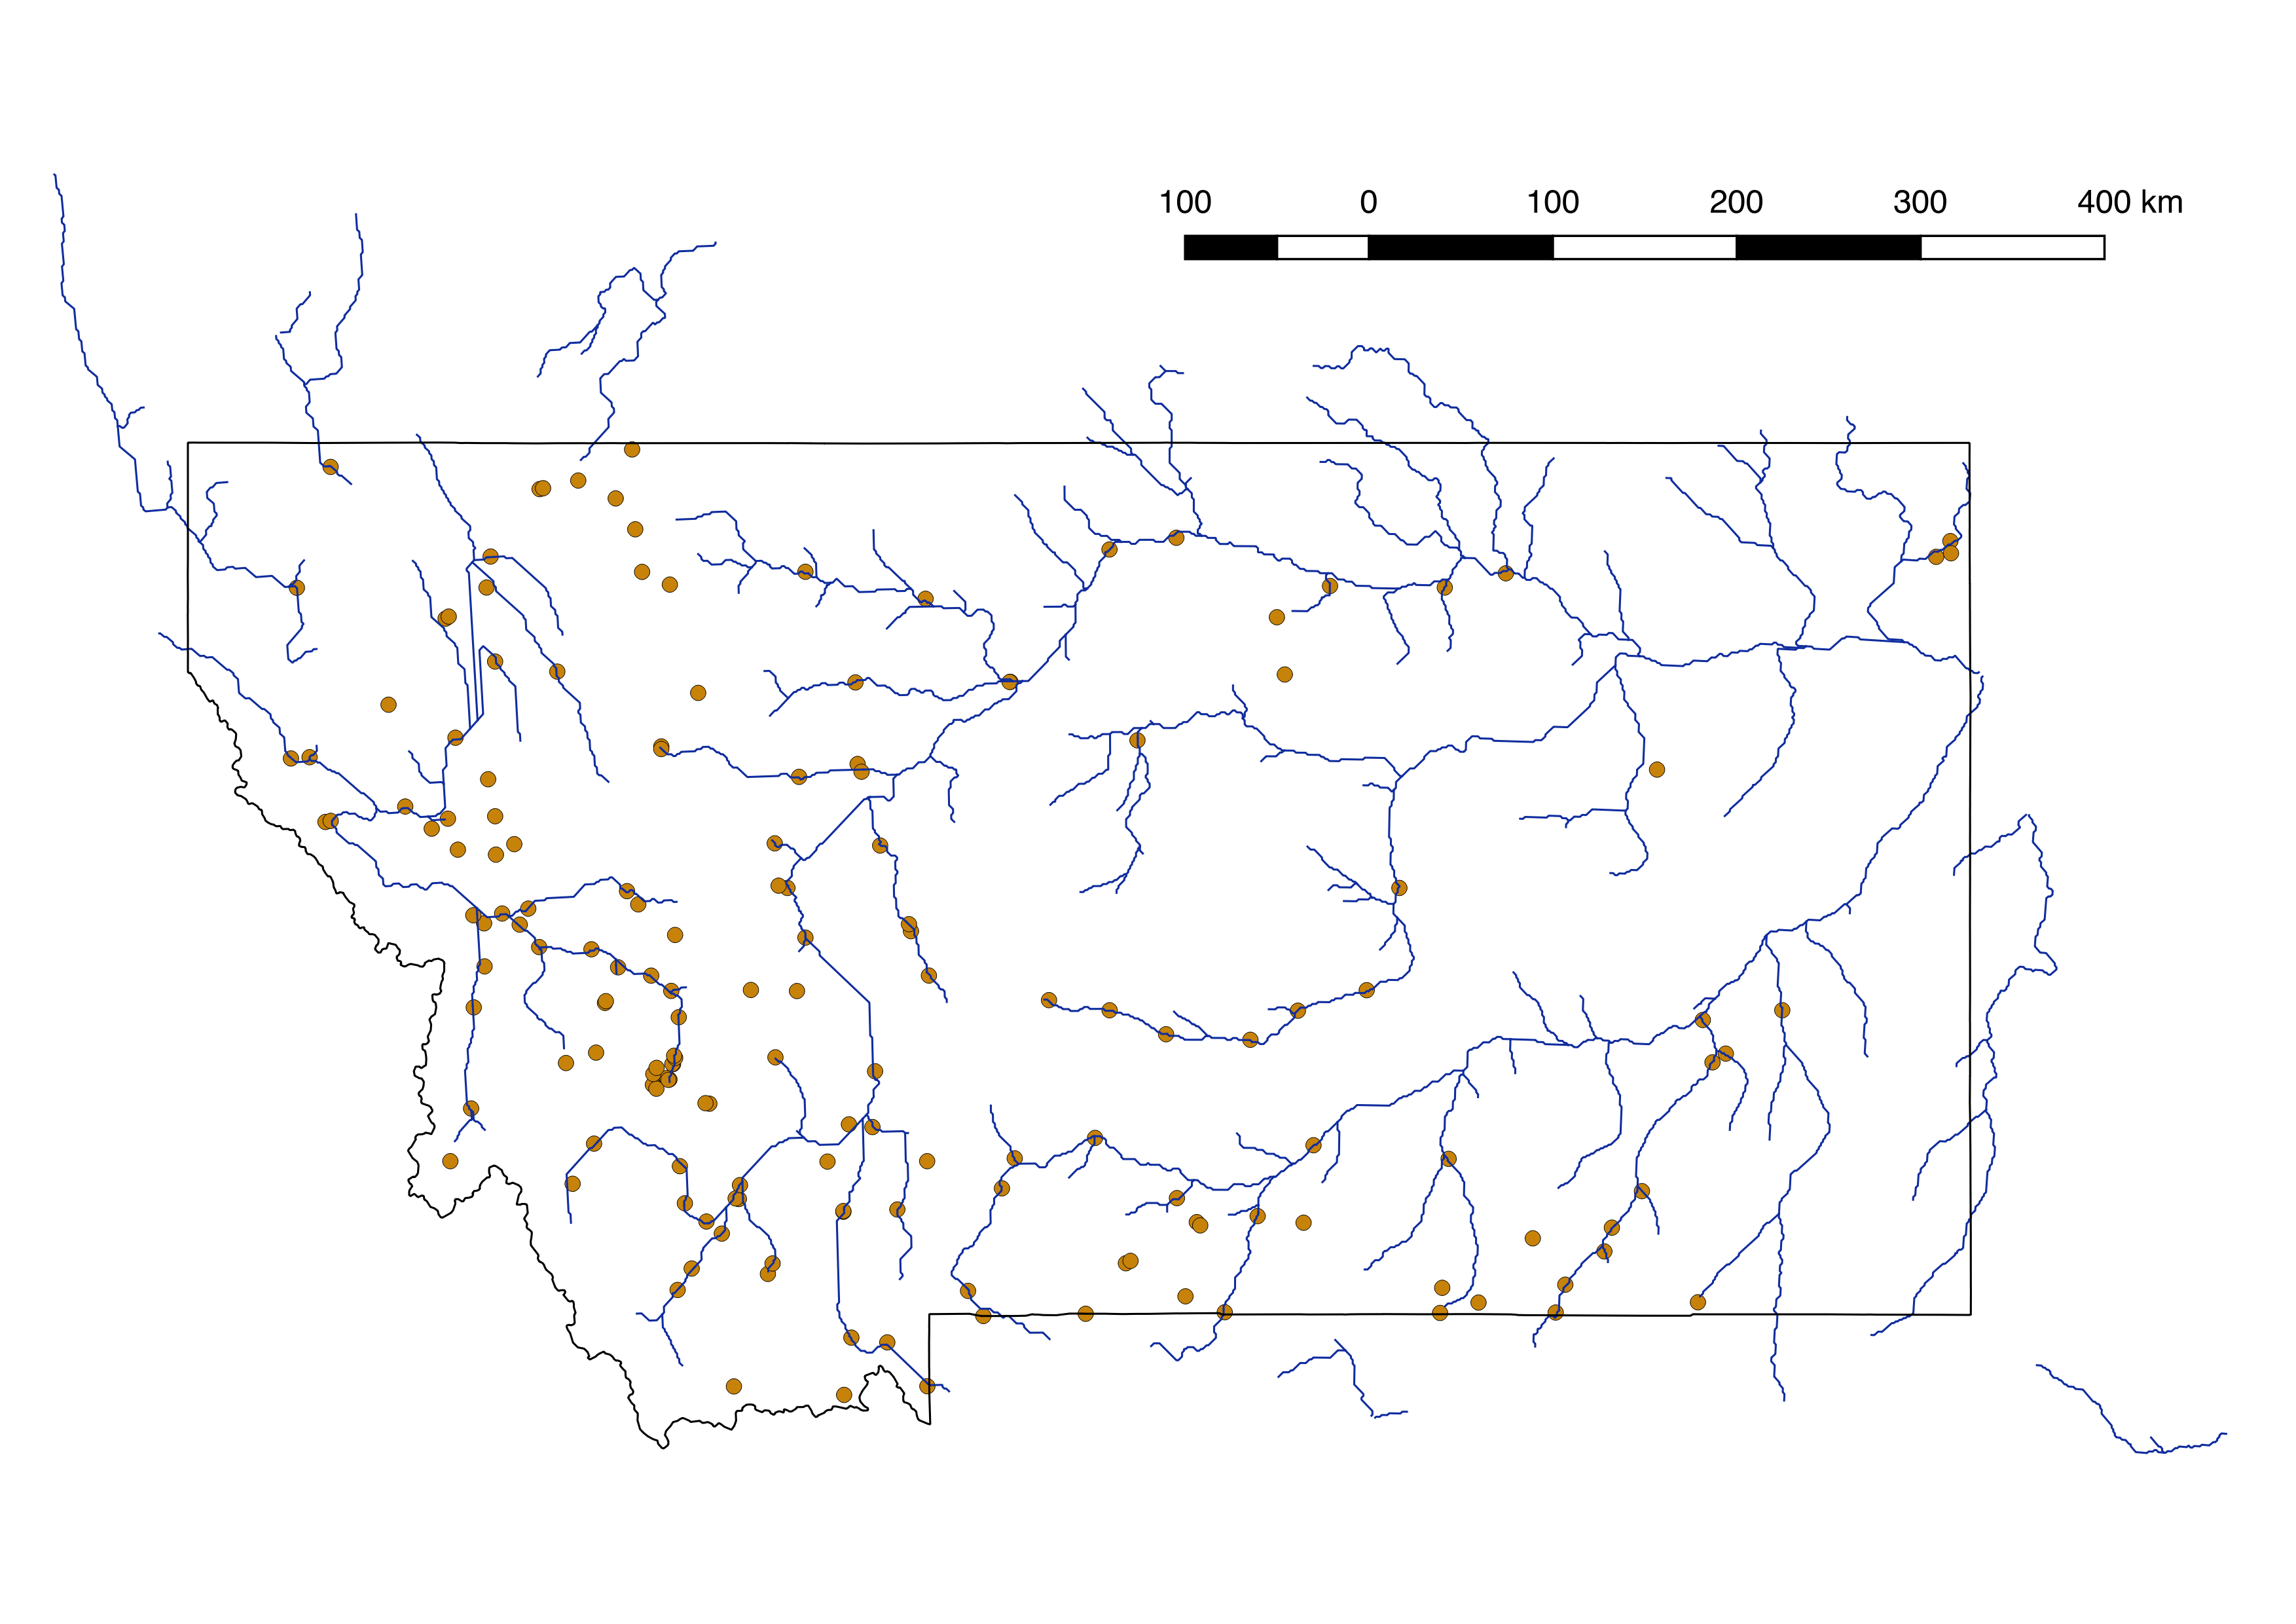
\includegraphics[width=0.95\textwidth]{stations}
    \caption{all \texttt{swe} stations (orange dots) and modeled streamflows}
    \label{fig:stations}
\end{figure}

\section{Catchment Data and Hierarchical Groups}

The hydrologic model utilizes the Watershed Boundary Dataset (WBD), a national hydrologic unit from the USGS that defines the areas of the United States landscape that drain to portions of the stream network, to separate Montana into 330 watersheds (Figure \ref{fig:huc8}.) Each watershed is associated with one of each type of parameter from Table \ref{tab:t_params}. These 330 watersheds fall into 3 larger watershed zones (called HUC4, or 4-digit hydrologic unit boundaries) that were utilized to classify each watershed into one of 3 hierarchical zones (Figure \ref{fig:huc4}.)

\begin{figure}[h]
    \centering
    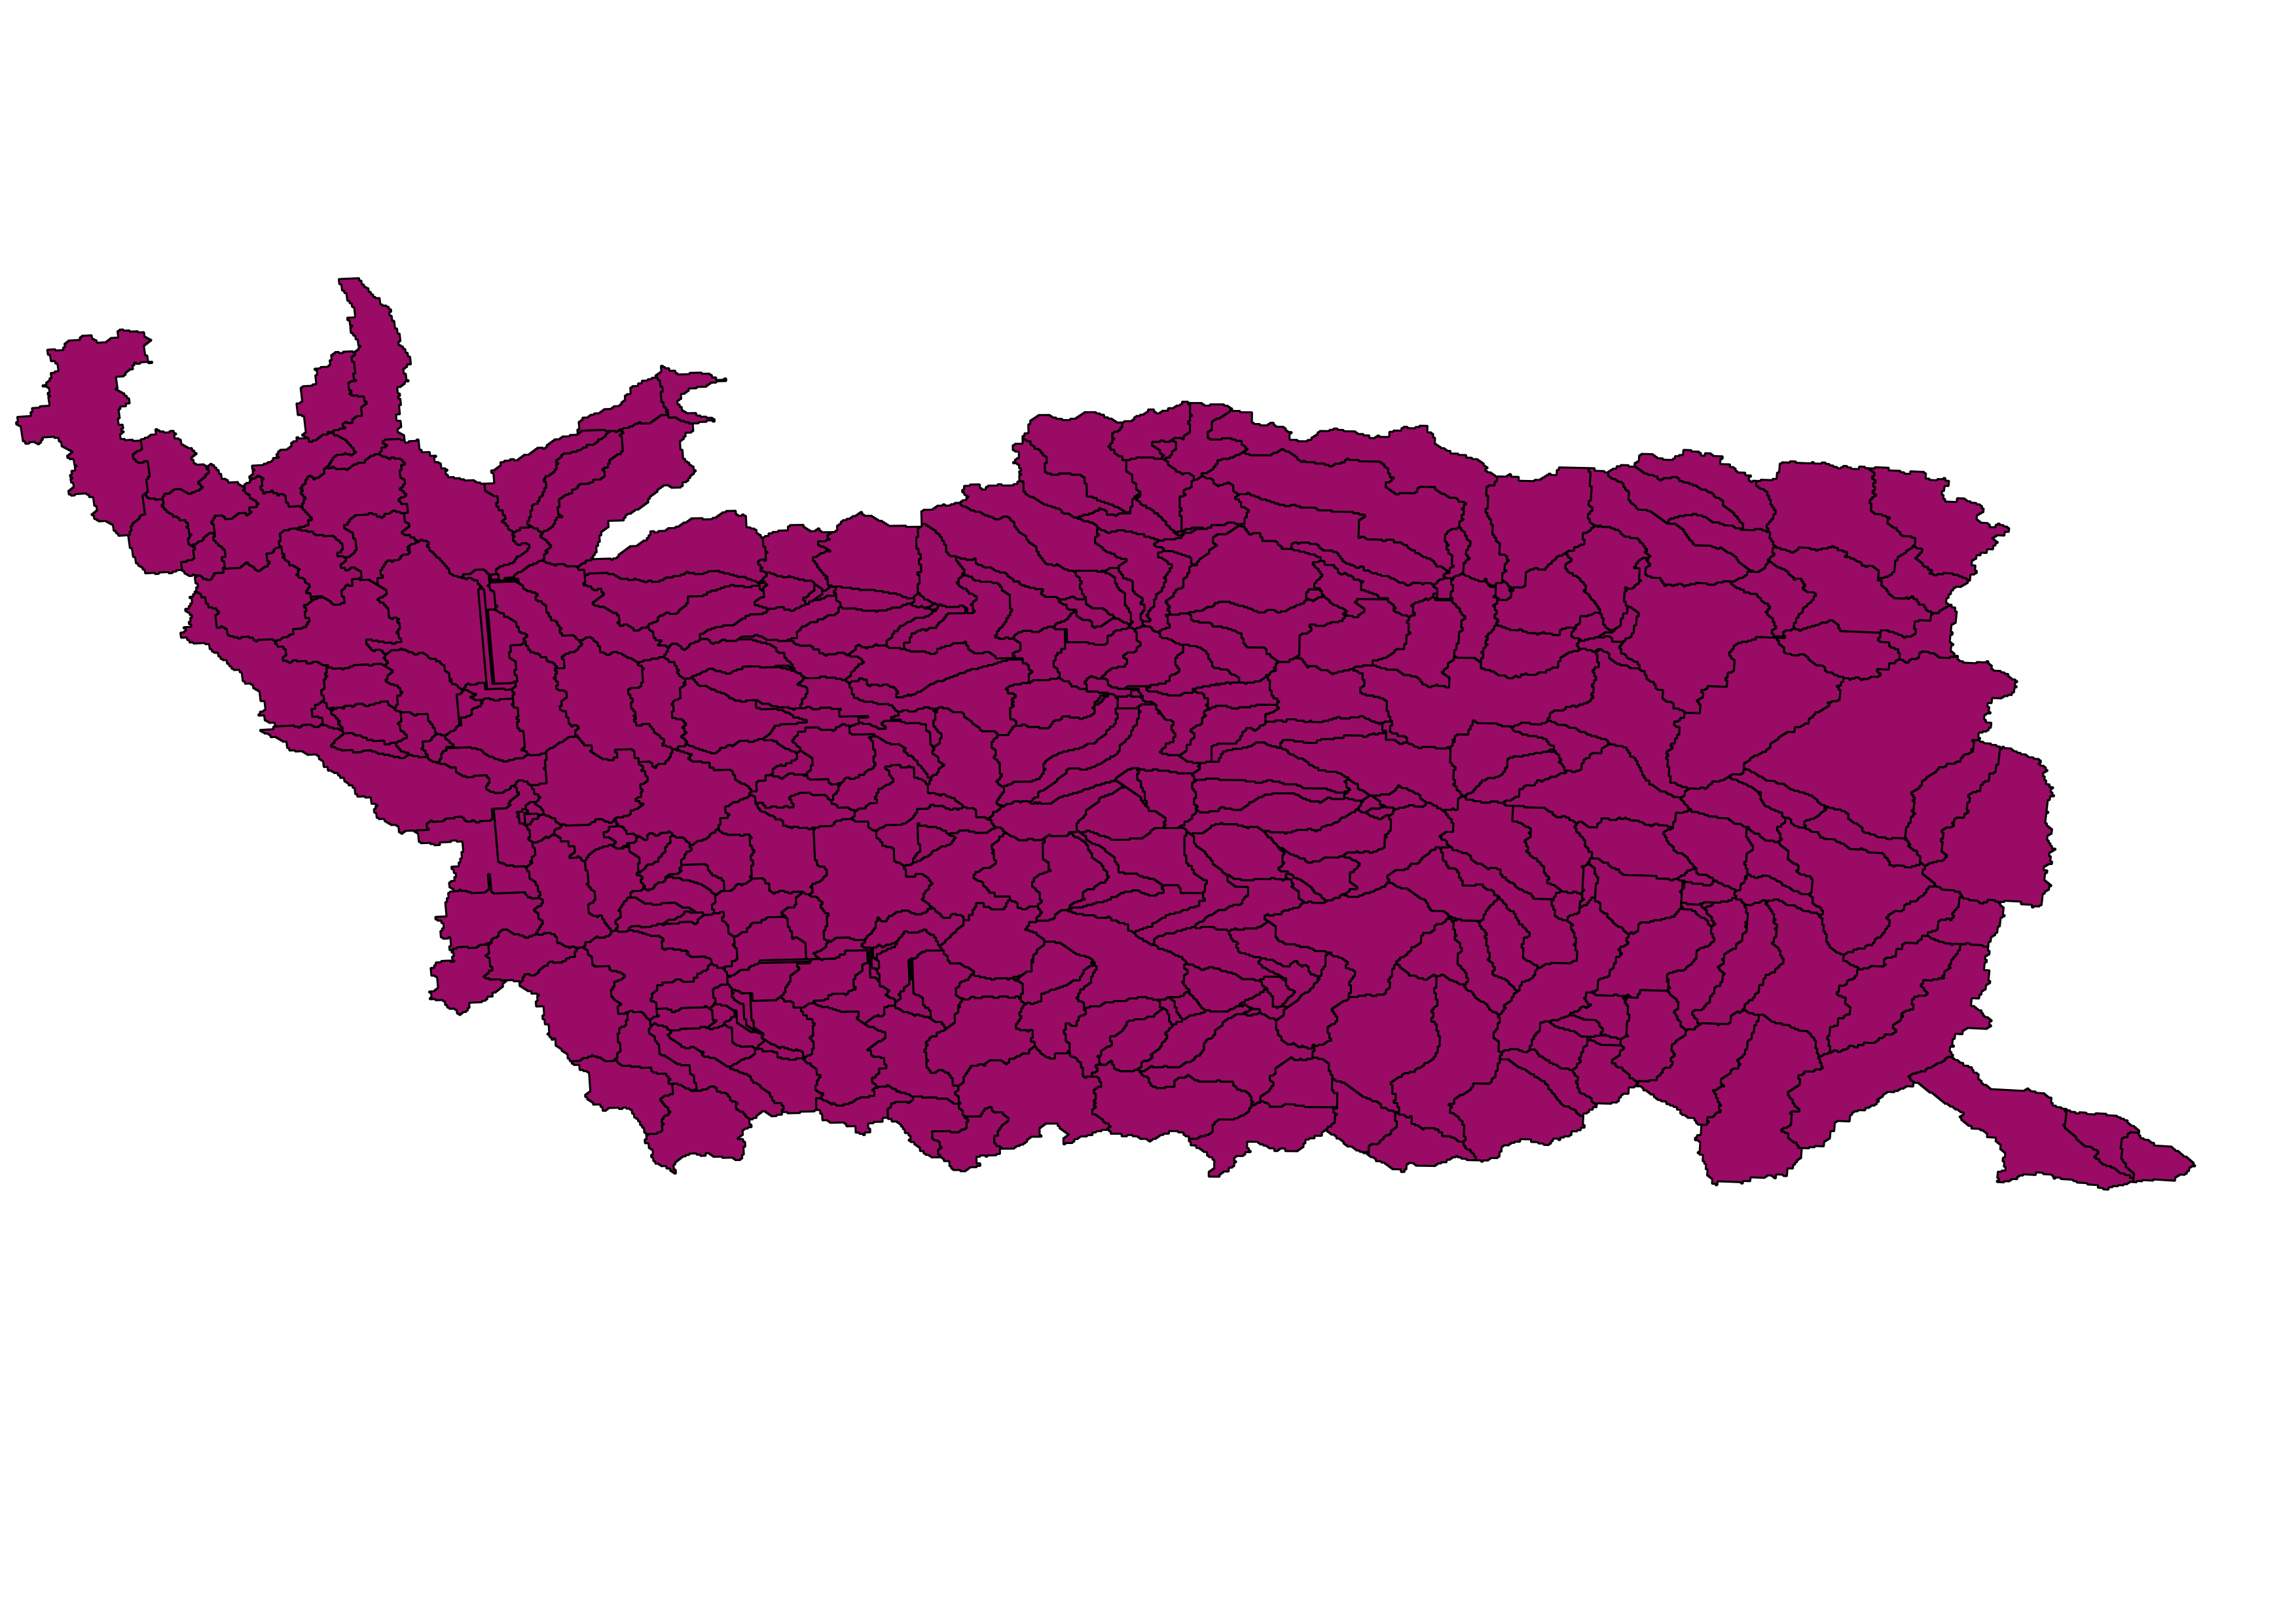
\includegraphics[width=0.95\textwidth]{huc8}
    \caption{Subbasins - HUC8 polygons}
    \label{fig:huc8}
\end{figure}

\begin{figure}[h]
    \centering
    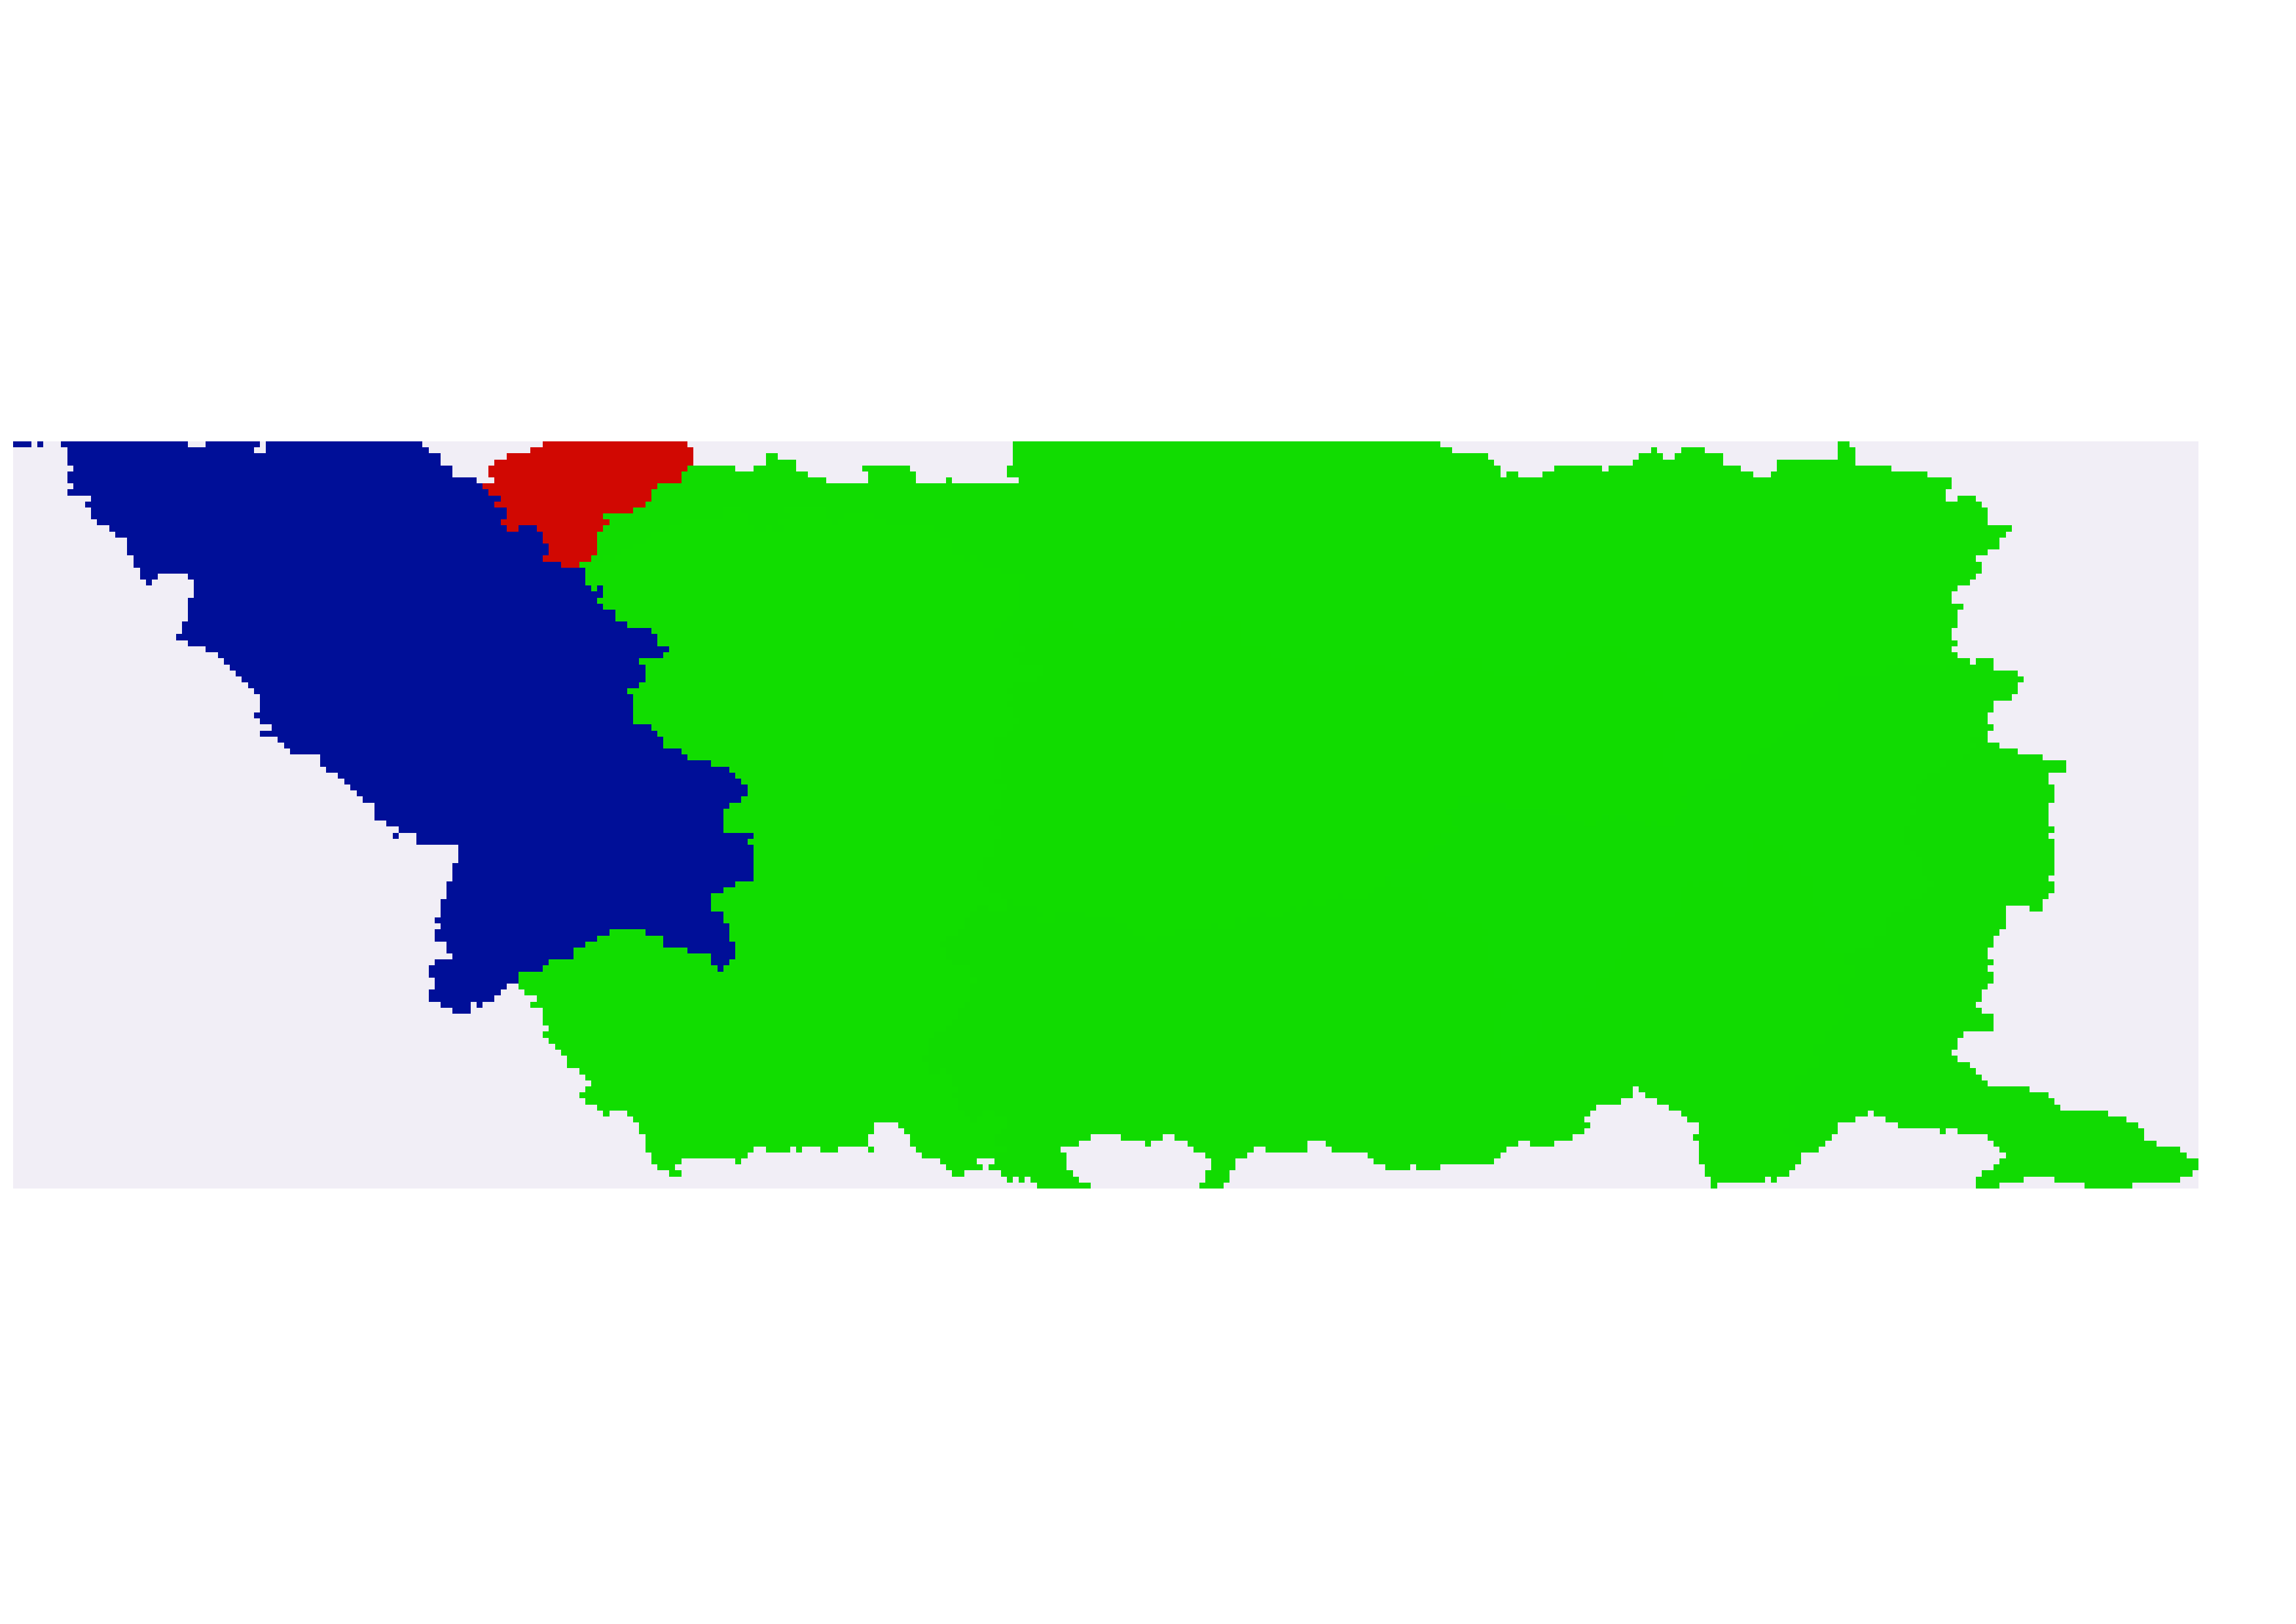
\includegraphics[width=0.95\textwidth]{huc4}
    \caption{Montana's 3 HUC4 zones rendered onto the raster grid.}
    \label{fig:huc4}
\end{figure}

\section{Filter Modifications}

The DHEnKF filter was implemented with a series of modifications that streamlined the filtering process.

\subsection{Parameter Ranges}

Parameter minimums and maximums were implemented on each model parameter to avoid anomalous or erratic model output such as negative snowfall or streamflow. The use of parameter bounds in Kalman filters is well researched and they have been used in a variety of past studies \cite{Shi2014}.


For every parameter $\theta$ a minimum $\theta_{min}$ and a maximum value $\theta_{max}$ was defined. If an ensemble member $i$ was generated outside of the range ($\theta_{min}$, $\theta_{max}$) during the apriori phase it was adjusted to:



\begin{align}\label{eq:boundary_eq}
\theta^{i} &= \left\{
\begin{array}{ll}
\theta_{min} & \theta^{i} < \theta_{min} \\
\theta_{max} &  \theta^{i} > \theta_{max} \\
\end{array}
\right.
\end{align}

\begin{align}\label{eq:boundary_eq_2}
\theta^{i} &= \left\{
\begin{array}{ll}
\theta_{min} & \theta^{i} < \theta_{min} \\
\theta_{max} &  \theta^{i} > \theta_{max} \\
\end{array}
\right.
\end{align}

For posterior parameters the same clipping logic from Eq. \eqref{eq:boundary_eq_2} is used. Initially an approach similar to the approach in \cite{Shi2014} was utilized, but this logic kept parameters immobile when the innovation between the state and observations were very large, rendering the filter's parameter correction phase  meaningless. To account for the problem of ensemble collapse, a minimum variance and a normalization feature was implemented (see below.)

\subsection{Normalization Feature}

To reduce erratic parameter ensemble behavior when sudden large discrepancies between observed data and model data appeared, a normalization feature was implemented in the parameter correction phase. For every parameter parameter $\theta$ a maximum movement range $\theta_{range}$ was defined based upon boundaries $\theta_{min}$ and $\theta_{max}$. An empirical parameter $\gamma$ controlled the maximum amount of movement per correction phase. 

\begin{equation}\label{eq:max_movement_thetarange}
\theta_{range} = \gamma(\theta_{max} - \theta_{min})
\end{equation}

\begin{align}\label{eq:max_movement}
\theta^{+} &= \left\{
\begin{array}{ll}
\theta^{+} & \theta^{+} > \theta^{-} - \theta_{range}, \theta^{+} < \theta^{-} + \theta_{range}  \\
\theta^{-} - \theta_{range} & \theta^{+} < \theta^{-} - \theta_{range} \\
\theta^{-} + \theta_{range} & \theta^{+} > \theta^{-} + \theta_{range} \\
\end{array}
\right.
\end{align}


$\gamma = 1$ allows for unhindered movement for theta, while $\gamma = 0$ does not allow any movement. For the purposes of this paper $\gamma = .1$ greatly reduced filter instability while allowing parameters to converge relatively quickly to far away values.

\section{Small Testset}

A filtering run could take anywhere between 20 hours and a week depending on calibration duration and number of ensembles used. In order to efficiently test new equations and starting parameters a small 3 node dataset was developed. This dataset covered the Bitterroot area of Montana and only held 3 subbasins.